\documentclass{article}

% if you need to pass options to natbib, use, e.g.:
% \PassOptionsToPackage{numbers, compress}{natbib}
% before loading nips_2016
%
% to avoid loading the natbib package, add option nonatbib:
% \usepackage[nonatbib]{nips_2016}

%\usepackage{nips_2016}

% to compile a camera-ready version, add the [final] option, e.g.:
\usepackage[final]{nips_2016}

\usepackage[utf8]{inputenc} % allow utf-8 input
\usepackage[T1]{fontenc}    % use 8-bit T1 fonts
\usepackage{hyperref}       % hyperlinks
\usepackage{url}            % simple URL typesetting
\usepackage{booktabs}       % professional-quality tables
\usepackage{amsfonts}       % blackboard math symbols
\usepackage{nicefrac}       % compact symbols for 1/2, etc.
\usepackage{microtype}      % microtypography
\usepackage{mathtools}
\usepackage{rotating}

\DeclareMathOperator*{\argmin}{arg\,min}
\DeclareMathOperator*{\argmax}{arg\,max}

\title{Contextual Pitch Prediction With \\Mixture Density Networks}

% The \author macro works with any number of authors. There are two
% commands used to separate the names and addresses of multiple
% authors: \And and \AND.
%
% Using \And between authors leaves it to LaTeX to determine where to
% break the lines. Using \AND forces a line break at that point. So,
% if LaTeX puts 3 of 4 authors names on the first line, and the last
% on the second line, try using \AND instead of \And before the third
% author name.

\author{
   Ryan McKenna, Qianxin Xu, Timm Allman\\
  School of Computer and Information Science\\
  University of Massachusetts, Amherst\\
  Amherst, MA 01002\\
  \texttt{\{rmckenna, qxu, tallman\}@cs.umass.edu} \\
}

\begin{document}
\maketitle 
\begin{abstract}
Understanding how a pitcher will behave in a particular situation can improve our ability to effectively model at bats. This motivates us to develop statistical models that explain the characteristics of pitches, including the type and location, based on the context in which the pitch was thrown. In this paper, we develop and introduce models that are designed to solve this problem. Specifically we model the context-dependent joint distribution $ f_C(type, x, y) $ using neural networks. We show that our models outperform simpler models that don't account for context, as well as other approaches based on machine learning.
\end{abstract}

\section{Introduction}

Mathematics has fundamentally changed the way baseball teams make decisions. Sabermetrics, the empirical analysis of baseball data, has provided teams with the formal tools they need to make more well-informed decisions. There is a vast amount of baseball data available, and this data has been used in many interesting ways, including for visualization, evaluating player performance, and making predictions about future events. This data contains an abundance of information that teams can use to make actionable decisions, but the information can only be used once the right tools are developed to model the data.

In this work, we develop models of pitchers' behavior. In particular we aim to model the distribution of pitch types and locations for a particular context, where the context consists of available and relevant information known before the pitch is thrown. With these models in hand, statisticians can more effectively model at bats and predict their outcomes. Furthermore, batters can utilize this information to better prepare for certain pitches depending on the context they are in.  

\section{Background}

\subsection{Existing Methods}

There are several studies about pitch analysis; Ganeshapillai and Guttag (Ganeshapillai and Guttag, 2012)\cite{ganeshapillai2012predicting} show that pitchers are much more predictable in counts that favor the batter. They use a linear support vector machine (SVM) to perform binary (fastball vs. nonfastball) classification on pitches of unknown type for each pitcher. They obtain an average prediction accuracy of roughly 70 percent across all pitchers.

Researchers have formulated the pitch type prediction task as a machine learning problem using classification algorithms.  Most of these researches use Support Vector Machine with a linear or Gaussian kernel to accomplish this task. Some studies also proposed the use of k-nearest neighbor to do the classification\cite{hamilton2014applying}.  They focus on the feature selection scheme that selects different features for different pitchers to improve the accuracy. 

This existing research was mainly focused on binary classification for pitch type. In this project, we are interested in the more general problem of obtaining the distribution over all pitch types and locations.  In this work, we propose several options for modeling these distributions and empirically evaluate them on over 3 million pitches from 2010-2014.  

\section{Models}

\subsection{The Data}

In order to understand the models, it is useful to know what data we are training them on, and exactly what features constitute the context that we frequently refer to.  Our data is collected from PITCH f/x, which is a pitch tracking system that tracks data on every pitch in every MLB game. Our models are trained and tested using PITCH f/x data from MLB games from 2010 to 2014. Each pitch in the data set includes a label for the $(x,y)$ location of the ball as it crossed home plate, and the type of the pitch (e.g., fastball, curveball) which is characterized based on the pitches' trajectory.  The data contains approximately 50 features, some of which are for book-keeping, and others which characterize the context of the pitch.  We select a subset of the relevant features and augment the data by deriving new and useful features from the original features.  Some of the features include the pitcher, the batter, the batter height and stance, the pitchers throwing hand, the count, the inning, the batters order in the lineup, flags for home/away and day/night, the day of the week, the month, the year, the home/away team, and the batter/pitcher team.  Some of these features may influence the type and location of a pitch more than others, and part of the challenge of developing good models is making them robust to noisy features.  Feature selection and preprocessing are important considerations in statistical modeling, so we compare 4 different features selection and standardization schemes for the pitch type prediction task, which will be described in more detail later.

\subsection{Model Decomposition}

We ultimately want to model the context-dependent joint distribution $ f_C(type, x, y) $, where $C$ is the context, $ type $ is a categorical random variable (fastball, curveball, changeup, etc.) and $ (x,y) $ are continuous random variables representing the location of the pitch as it crossed home plate.  This joint distribution can naturally be decomposed into the product of two distributions as shown in equation~\ref{decomp}.

\begin{equation} \label{decomp}
f_C(type, x, y) = P_C(type) f_C(x, y \mid type) \\
\end{equation}

We use the notation $ P_C(type) $ and $ f_C(x, y \mid type) $ to emphasize that the former is a probability mass function while the latter is a probability density function.  By decomposing $ f_C(type, x, y) $ in this way, we can model $ P_C(type) $ and $ f_C(x, y \mid type) $ separately and merge their results to recover the full joint distribution $ f_C(type, x, y) $.  

Modeling $ P_C(type) $ is a well-understood problem in the machine learning community.  It can be solved by using a probabilistic classifier, which aims to find a function mapping the context $C$ to a vector of probabilities over pitch types.  Several methods exist to find such a mapping, including Logistic Regression, Support Vector Machines with Platt Scaling, and Neural Networks. 

Modeling $ f_C(x, y \mid type) $ is more challenging and there is significantly less literature on this problem.  A significant contribution of this work is the development of a such a model.

In the following sections we will slightly abuse notation in order to more effectively get the important points across.  $ C_i $ is the context for example $i$, which we assume is a vector of real values.  $ type_i $ is the observed pitch type of example $i$.  $ (x_i, y_i) $ is the location of example $i$ as it crossed home plate.  When the subscript is omitted from an expression we are usually using the expression as a probability distribution.  When the subscripts are included, however, the expression refers to the pdf evaluated at the given point.  We use $ f $ in multiple places with different meanings, and its meaning should be clear based on the parameters and other context.  In general, we use $f$ to denote a pdf, and $P$ to denote a pmf.  

\subsection{The Baseline}

Establishing a baseline model is important to draw conclusions about the more complex models, and sometimes the simple models perform better anyway.  The baseline model makes the intuitive simplifying assumption that for each pitcher, every pitch $ (type, x, y) $ thrown was sampled from the same distribution $ f_{pitcher}(type, x, y) $ independent of all other context.  This assumptions applies to the decomposed distributions as well as shown in equation~\ref{baseline}.

\begin{equation} \label{baseline}
\begin{split}
P_C(type) &= P_{pitcher}(type) \\
f_C(x, y \mid type) &= f_{pitcher}(x, y \mid type)\\
\end{split}
\end{equation}

This natural assumption leads to one model per pitcher where each model is independently constructed using all the available data for that pitcher.  

\subsubsection{Categorical Distributions}

In modeling the pitch type for a particular pitcher, we are faced with the problem of maximizing the likelihood of the data, as shown in equation~\ref{mle-type}.

\begin{equation} \label{mle-type}
\hat{\theta} = \argmax_{\theta} \prod_{i=1}^N P(type_i \mid \theta)
\end{equation}

$P(type \mid \theta) $ is a categorical distribution parameterized by $ \theta $\footnote{$\theta$ is a vector of probabilities, one for each pitch type where $ P(type = j \mid \theta) = \theta_j $} and $ type_i $ is the observed pitch type for example $i$.  It is well known that $ \hat{\theta} $ can be computed in closed form as the empirical proportions of each pitch type in the data. 

In order to avoid over-fitting for pitchers with little data, it is important to use maximum a posteriori (MAP) estimation rather than maximum likelihood estimation.  In order to do that, we must introduce a prior distribution over the space of possible models.  The natural thing to do here is assume $ \theta $ is sampled from a Dirichlet distribution $ \theta \sim Dir(\alpha \bar{\theta}) $ where $ \alpha $ is a hyper-parameter to be tuned that determines the amount of influence the prior distribution has on the MAP estimate, and $ \bar{\theta} $ is computed from the sample data (for all pitchers combined) as the empirical proportions of each pitch type.  The solution to the MAP estimation problem is also well known, as shown in equation~\ref{map-type}.

\begin{equation} \label{map-type}
\begin{split}
\tilde{\theta} &= \argmax_{\theta} \prod_{i=1}^N P(type_i \mid \theta) f(\theta) \\
\tilde{\theta} &= \frac{\alpha \bar{\theta} + N \hat{\theta}}{\alpha + N}
\end{split}
\end{equation}

$ f(\theta) $ is the probability distribution of the Dirichlet distribution $ Dir(\alpha \bar{\theta}) $.  This intuitve result can be interpreted as taking the weighted average between the empirical proportions for a particular pitcher and the empirical proportions for all pitchers combined.

\subsubsection{Gaussian Mixture Models} \label{gmm}

We can approximate the pitch location distribution for a particular pitcher with a Gaussian Mixture Model (GMM), which is a commonly used model for parametric density estimation.  A GMM is parameterized by mixture weights $ \phi $, means $ \mu $ and covariance matrices $ \Sigma $ and its pdf is given in equation~\ref{gmm-pdf}.

\begin{equation} \label{gmm-pdf}
f(x, y \mid type) = \sum_{k=1}^K \phi_k^{(type)} f(x,y \mid \mu_k^{(type)}, \Sigma_k^{(type)})
\end{equation}

$ f(\cdot \mid \mu, \Sigma) $ is the pdf of a multivariate normal distribution.  A simple GMM with $K=3$ is shown in figure~\ref{example-gmm}.  

\begin{figure}
\centering
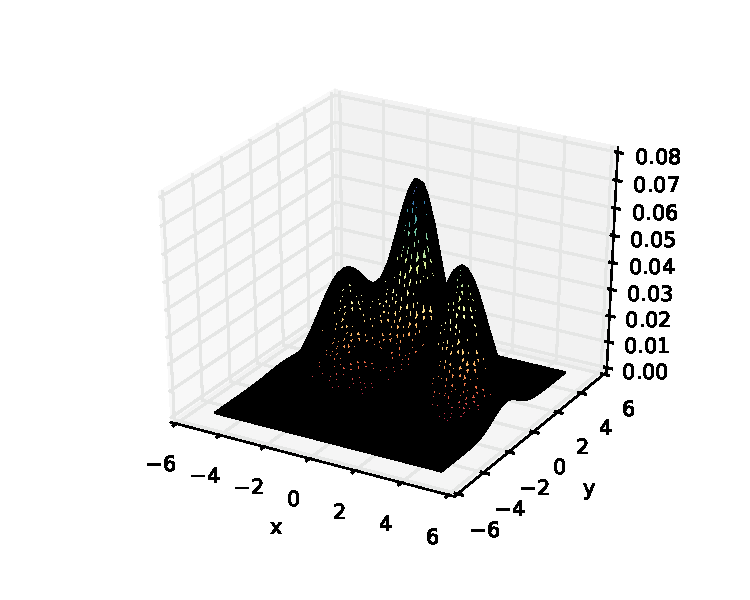
\includegraphics[width=\textwidth/2]{mixture-model}
\caption{A simple GMM with 3 mixture components.}
\label{example-gmm}
\end{figure}

We want to find the parameters that maximize the likelihood of the data, as shown in equation~\ref{mle-loc}

\begin{equation} \label{mle-loc}
\hat{\phi}, \hat{\mu}, \hat{\Sigma} = \argmax_{\phi, \mu, \Sigma} \prod_{i=1}^N f(x_i, y_i \mid type_i)
\end{equation}

$(x_i, y_i)$ and $type_i$ are the observed pitch characteristics of example $i$.  Unlike the model for pitch type, it is not generally possible to compute the MLE parameters of a GMM in closed form.  Usually, they are learned numerically with iterative algorithms such as expectation maximization or gradient descent instead.  Also, the global maximum is not always attainable since the log likelihood function is not concave, so we must usually accept local maximum instead.  

To avoid over-fitting, we introduce a simple heuristic motivated by the result from equation~\ref{map-type}.  Specifically, we compute the MLE parameters of a GMM for every pitcher in the data set separately, then we compute a global GMM model for all pitchers combined.  A new regularized model with double the number of mixture components is constructed for each pitcher by combining the models and scaling the mixture weights $ \hat{\phi}_k \leftarrow \frac{N}{N+\alpha} \hat{\phi}_k $ for the pitcher specific model and $ \hat{\phi}_k \leftarrow \frac{\alpha}{N+\alpha} \hat{\phi}_k $ for the global model.  $ \alpha $ is a hyperparameter that needs to be tuned so that the model generalizes well. 

\subsection{Neural Networks}

The main problem with the baseline models introduced in the previous section is that they ignore possibly relevant context including the batter, his height and stance, and the count.  One could generalize the methods described in the baseline model to produce a context-specific model rather than a pitcher-specific model.  However, the number of data points available for a specific context decays exponentially with the number of context features we use.  Since the available data for each model is limited, the models wouldn't be very enlightening.  

This inspires us to develop a better approach based on neural networks.  Specifically, we assume that each $ (type, x, y) $ is sampled from some parametric distribution (categorical distribution for $ type $, GMM for $ (x,y) $) where the parameters of the distribution are a function of the context $C$.  The challenge is then to automatically learn the complex, nonlinear, and unknown dependence between $C$ and the model parameters.  We use neural networks to automatically learn these dependencies from the data.  

The benefits of this approach are two-fold.  First, we can use all of our context features without worrying about over-fitting; the neural network will automatically be able to learn which features are relevant.  Second, since neural networks generalize to new contexts effectively, so we don't have to regularize with some global model.  

\subsubsection{Neural Network Classifier}

As with the baseline model, we seek to maximize the likelihood of the data as shown in equation~\ref{nnet-type}, but this time we are maximizing with respect to a parametric function $ \theta_w $ which maps the context to a probability vector, such as a neural network with weights $w$.  Also, instead of building one model per pitcher, we are building one global model, where the pitcher is included as one of the features in the context.  This allows information sharing to occur between two different pitchers, which wasn't possible with the baseline models.  

\begin{equation} \label{nnet-type}
\hat{w} = \argmax_{w} \prod_{i=1}^N P(type_i \mid \theta_w(C_i))
\end{equation}

Finding $ \hat{w} $ is a matter of fitting a neural network to the data using the negative log likelihood as the loss function.  This problem is well understood among people familiar with machine learning so we will leave out the niceties.  

\textbf{Implementation Details}

We convert the categorical data to a one hot encoding and use embeddings\cite{Mikolov:2013:DRW:2999792.2999959} to represent the pitchers and batters as vectors in $d$-dimensional space.  Using a one hot encoding for the pitcher and batter would only work if representing the data as a sparse matrix, since there are thousands of players and millions of training examples.  
We configure the neural network to have a tunable network structure.  We also regularize the model by using dropout and the early stopping heuristic.  We optimize the network weights using the Adam optimizer, which we found was more robust to the learning rate than stochastic gradient descent, and it converged to a good solution much faster.  The hyper-parameters of our model are shown below, and we explore the space of hyper-parameters using a randomized search.  In general, our design decisions were guided by the tips provided in \cite{Goodfellow-et-al-2016-Book}.
\begin{itemize}
\item \textbf{learning rate} for stochastic optimizer
\item \textbf{batch size} for stochastic optimizer
\item \textbf{player embedding size}
\item \textbf{hidden layers} to specify network structure
\item \textbf{activation function}
\item \textbf{dropout rate} for regularization
\item \textbf{patience} for early stopping heuristic
\end{itemize}

\subsubsection{Mixture Density Network} \label{mdn-section}

\begin{figure}
\centering
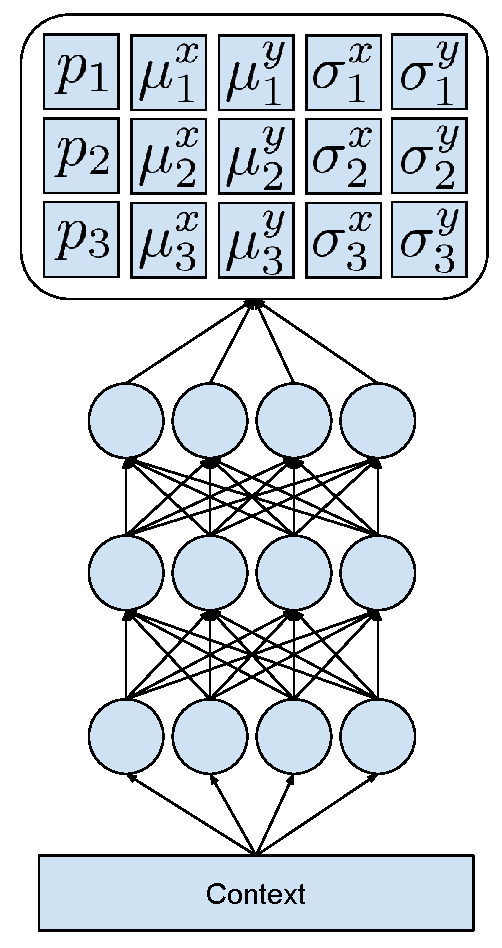
\includegraphics[angle=-90,width=0.75\textwidth]{mdn}
\caption{A simple Mixture Density Network with 3 mixture components.}
\label{example-mdn}
\end{figure}

Since the location $(x,y)$ of a pitch is continuous, classifiers are not suitable for modeling it.  Usually when the output is continuous, it is common to use regressors instead.  However, regressors only produce a single prediction for each input, and the location of the pitch a highly uncertain quantity, even when the context is known.  Pitchers usually use a randomized policy when deciding where to throw the next pitch, because batters can easily exploit them if they are too predictable.  Thus, it's better to directly model our uncertainty about the location of the next pitch as a probability distribution over all possible locations.  As described in section~\ref{gmm}, Gaussian Mixture Models are a good way to parameterize our uncertainty about the location of the next pitch.

In order to combine the benefits of GMMs and neural networks, we use Mixture Density Networks which are neural networks where the output neurons are interpreted as parameters to a GMM \cite{Williams:1996:UNN:1362161.1362171}.  The neural network is just a function  mapping the context $C$ to GMM parameters $ \phi_k, \mu_k $, and $ \Sigma_k $.  We make the simplifying assumption that $ \Sigma_k $ is diagonal, meaning that we only have to learn $ \sigma_{xx} $ and $ \sigma_{yy} $, although it is relatively straightforward to remove that assumption by introducing more output neurons $ \sigma_{xy} $ that need to be learned.  

Maximizing the likelihood of the data is the objective of our model.  Let $ f(x, y \mid \phi_w(C), \mu_w(C), \Sigma_w(C)) $ denote the pdf of a GMM with mixture weights $ \phi_w(C) $, means $ \mu_w(C) $, and covariance matrices $ \Sigma_w(C) $, where the context $C$ now includes the pitch type since we are modeling $ f_C(x,y \mid type) $.  $\phi_w, \mu_w, $ and $ \Sigma_w $ are all functions of the context, which are parameterized by $w$ - the weights of the neural network.  In order to ensure that the probability distribution produced by the network is valid, we use the softmax function on the output neurons associated with $ \phi_w(C) $, and we use an exponential function on the output neurons associated with $ \Sigma_w(C) $.

Our goal is to maximize the context-dependent likelihood of the data, as shown in equation~\ref{nnet-loc}.  We do that by training a neural network with the negative log likelihood as the loss function.  This is done by taking the neural network outputs for each training example, constructing a GMM with the given parameters, then evaluating that pdf on the $(x,y)$ location of that training example.  

\begin{equation} \label{nnet-loc}
\hat{w} = \argmax_{w} \prod_{i=1}^N f(x_i, y_i \mid \phi_w(C_i), \mu_w(C_i), \Sigma_w(C_i))
\end{equation}

We use the same feature representation as before, and we have the same hyperparameters as before, as well as a new hyperparameter for the number of mixture components.  However, this model is significantly more expensive to train because the loss function is more computationally intensive to evaluate than before, so our search over the space of hyperparameters only consisted of a few experiments, which were largely influenced by the best hyperparameters in the network for pitch type.  This Mixture Density Network gives us an approximation of the pitch location distribution for any conceivable context, even if there is little or no training data for that context.

Both neural networks were constructed using TensorFlow \cite{tensorflow2015-whitepaper}, as it gave us full control over the inner workings of the neural networks.  

\subsection{Other Methods}

While there aren't many other well-known ways to model $ f_C(x, y \mid type) $, there are several other models we could use for $ P_C(type) $.  Any classification algorithm that can produce well calibrated probability estimates is suitable for this task.  We empirically evaluate Logistic Regression, Support Vector Machines and Random Forests on this problem. 

We implemented a linear SVM with soft margins to compare the performance of the neural network model. The binary SVM computes a decision function $f(x)$ such that $sign(f(x))$ can be used to predict the label of the test example. However, we want to get the classes probability, so we convert the SVM scores to probability estimates using Platt scaling, which approximates the posterior probability by a sigmoid function\cite{lin2007note}. Then we estimate the multi-class probability by combining the pairwise class probabilities\cite{wu2004probability}.  Due to our large data size, we use stochastic gradient descent (SGD) to find the parameters of the SVM. We also implemented the Random Forest classifier and Logistic Regression classifier with stochastic gradient descent and stochastic average gradient algorithms to compare their performance.  These models were all constructed in scikit-learn \cite{scikit-learn}, which provided us with a clean interface to quickly and easily test out various machine learning algorithms.  

\section{Results}

\begin{table}[thb]
\centering
\begin{tabular}{|c|c|}
\hline
\multicolumn{2}{|c|}{$P_C(type)$} \\ \hline
Model                 & Score \\\hline
Baseline              & 1.30  \\
Logistic Regression   & 1.26  \\
SVM                   & 1.32  \\
Neural Network        & 1.15  \\\hline
\end{tabular}
\quad
\begin{tabular}{|c|c|}
\hline
\multicolumn{2}{|c|}{$f_C(x,y \mid type)$} \\ \hline
Model                   & Score \\\hline
Baseline                & 2.40  \\
Mixture Density Network & 2.28  \\\hline
\end{tabular}
\caption{Average negative log likelihood for each model} \label{results-table}
\end{table}

We evaluate the quality of our models by splitting our data into a training set ($\sim 2.6$ million examples) and a test set ($\sim 850$ thousand examples) then computing the negative average log-likelihood evaluated on the test set (lower scores are better).  We feel this is the best metric to use because it measures how well the whole distribution is modeled, rather than whether the most likely predicted occurrence was observed.  The results of these tests are shown in table~\ref{results-table}.  From these results, one can easily see that the neural network worked the best for both modeling problems.  However, it's not immediately obvious how to interpret these results: is the neural network significantly better than the baseline or is it a small improvement? By computing the geometric mean of the likelihood ratio between the neural network and the baseline model on the test set, we can answer that question.  For the pitch type modeling task, the likelihood ratio is $ e^{1.30-1.15} \approx 1.16 $ which means on average, the likelihood of making a particular observation is $1.16$ times higher under the neural network model than under the baseline model.  Similarly for the pitch location modeling task, the likelihood ratio is $ e^{2.40 - 2.28} \approx 1.13 $.  This gives us a more intuitive sense of the performance different between the baseline models and the neural networks.  This basically means that if the baseline model predicted the correct pitch type to occur with probability $0.5$, then the neural network would have predicted it to occur with probability $1.16 \cdot 0.5 = 0.58$ on average.  While this improvement may seem small, it is important to remember that the baseline model is already pretty good; also, there is an upper bound to how well one can predict the type and location of the next pitch, because if pitchers become too predictable they are easy to exploit.  Our models establish a solid benchmark for this problem, from which future methods can be compared.  

\subsection{Neural Network Architecture}

Optimizing the neural network hyperparameters proved to be very important to achieve good performance.  Specifically, we found that the initial learning rate for the stochastic gradient descent optimizer was a very important hyperparameter. However, once we switched to the Adam optimizer, we found that the default learning rate worked quite well: it converged to a solution in many fewer iterations than SGD, and it was relatively robust to other learning rates as well.  We found that early stopping helped avoid over-fitting, and that using small dropout rate of $ 0.1 $ worked the best empirically.  We also found that in general, deeper networks produced better models, but that three hidden layers was usually enough to reach the best score.  We found that a mini batch size of about 2000 training examples for the stochastic optimizer worked well compared to other batch sizes.  Finally, we found that the size of the player embedding should be about 50.  The architecture specified in this section worked the best for the pitch type modeling task, and we used these results to influence our network architecture for the more expensive model of pitch location. Doing a more thorough exploration through the hyperparameter space for that model may be worthwhile.

\subsection{Feature Representation}

Feature representation was a very important consideration in this work.  We show that when the features are not preprocessed effectively, the machine learning algorithms can't even overcome the performance of the baseline model.  

The random forest, logistic regression, and SVM models use two sets of data: ``original'' and ``computed''. The original dataset includes the features pitcher, batter, away team, home team, year, batter handedness, pitcher handedness, inning half, batter team, pitcher team, inning, batter position in the order, weekday, month, balls, strikes, whether it's a night game, whether the batter is batting for the home team, the top of the strike zone, and the bottom of the strike zone. The computed dataset consists of pitcher-batter prior for each type of pitch (which is computed as an empirical proportion on the training set), whether the pitcher and batter have the same handedness (1 feature), inning, balls, strikes, whether it's a night game, and whether the batter is batting for the home team. This feature choice is motivated by previous work\cite{ganeshapillai2012predicting}. For each of these preprocessed data sets the non-categorical features can either be left as is or be ``standardized'' by scaling the data to have zero mean and unit variance.

\begin{table}[ht]
	\centering
	\begin{tabular}{ | l || l | l | l | l |  } %p{5mm}
		\hline
		Model         & Original & Original standardized & Computed & Computed standardized\\\hline
		Random Forest & 1.474    & 1.479                 & 1.442    & 1.443 \\\hline
        SVM-L         & 1.333    & 1.905                 & 1.481    & 1.458 \\\hline
        LR with SGD   & 1.425    & 1.268                 & 1.420    & 1.423 \\\hline
        LR with SAG   & 1.258    & 1.257                 & 1.493    & 1.493 \\\hline
	\end{tabular}
    \caption{Log-likelihood comparison over different models and feature sets}
	\label{tab:two}
\end{table}

\begin{table}[ht]
	\centering
	\begin{tabular}{ |l || l | l | l | l |  } %p{5mm}
		\hline
		Model         & Original & Original standardized & Computed & Computed standardized\\\hline
		Random Forest & 884      & 858                   & 456      & 293  \\\hline
        SVM-L         & 1800     & 1259                  & 815      & 1204 \\\hline
        LR with SGD   & 1911     & 2086                  & 459      & 426  \\\hline
        LR with SAG   & 585      & 7474                  & 1625     & 1416 \\\hline
	\end{tabular}
    \caption{Wall time (seconds) comparison over different models and feature sets}
	\label{tab:three}
\end{table}

Table 2 describes the average negative log-likelihood over different classifiers under different feature sets.  The feature choice seems to have little impact on the random forest classifier, while more substantially impacting the SVM and logistic regression models.
Table 3 depicts the training time over different classifiers and feature sets. This data was collected on a machine with an Intel Core I7-4900mq. For Random Forest classifier while the accuracy doesn't depend on feature selection the performance does. The SVM and Logistic classifiers deeply depends on the feature representation for good performance, as well as accuracy. For comparison the classification neural net takes about 1300 seconds to train on an Intel Core I7-4790K, while the logistic regression with SAG on the original features takes 260 seconds and the baseline model takes just 3. 
From these experiments, we understand how important feature representation, model selection and optimization algorithm are. For pitch type prediction, Logistic Regression with stochastic average gradient (SAG) which use the original feature set (one-hot encoding of categorical features) is good choice based on our experiments if speed of training is an issue.  It outperforms the baseline model in terms of log likelihood, but even the baseline model is decent and can be trained extremely quickly. If accuracy is the goal than our neural net outperforms the logistic regression model at the cost of increased training time.  Also, the neural networks are general enough to work for both the pitch type modeling task and the pitch location modeling task.  

\section{Conclusions and Future Work}

In this work, we demonstrated that we can more effectively model the distribution of pitch types and locations by using neural networks to map context features to probability distributions.  Specifically, we showed that neural networks are well suited for modeling the context dependent distribution $ P_C(type) $, as they outperformed our baseline model and other probabilistic classifiers such as Logistic Regression and Support Vector Machines.  We also found that Mixture Density Networks are well suited for modeling the context-dependent conditional distribution $ f_C(x, y \mid type) $.  

There are several ways this work can be extended.  Some of these ideas are exploratory while others we are confident can improve the predictive performance significantly.  The data set we used in this work only contained a limited number of contextual features.  By merging our data with other data sets, or deriving new features from the data we already have, the neural network can learn new dependencies between the context features and the parameters of the distributions.  Some of the features which we believe may help the predictive performance are the current score, the men on base, and the number of pitches thrown by the pitcher in the current game.  We also believe the previous few pitches, including their type, location, and outcome (ball, strike, foul, etc.) would be strongly correlated with the network outputs, although these features are not currently included in our data set.  While simply making these features should work well, a more principled approach to leveraging this information is by partitioning the data into at bats, where each at bat is just a sequence of pitches, and modeling the sequence data with recurrent neural networks.  The mixture density network architecture described in section~\ref{mdn-section} can easily be applied to recurrent neural networks, and so we believe this is one of the more promising avenues for future work.  

We would like to empirically analyze the importance of the different features.  Among the included features, we believe that the pitcher, the batter height and stance, and the current count are among the most important features.  We would also like to more thoroughly explore the space of hyperparameters in the hopes of improving the predictive performance of our models.  This work has been made available on GitHub at \url{https://github.com/ryan112358/pitch-prediction}.

\bibliographystyle{plain}
\bibliography{references}
\end{document}